% !TeX program = xelatex
% Approved increment: textbook sections 1.6, 1.7, and 1.8.
\documentclass[12pt,a4paper]{article}
\RequirePackage{array}[=2024-06-01]
% !TeX root = ../2/main.tex
\usepackage[a4paper,margin=25mm,headheight=16pt]{geometry}
\usepackage{amsmath,amssymb}
\usepackage{graphicx}
\usepackage{booktabs}
\usepackage{tabularx}
\usepackage{siunitx}
\usepackage{tikz}
\usepackage{circuitikz}
\usepackage[unicode,hidelinks]{hyperref}
\usepackage{xepersian}
% Only the regular B Nazanin file is installed; synthesize bold explicitly.
\settextfont[Path=C:/Windows/Fonts/,AutoFakeBold=2,AutoFakeSlant=0.2]{B-NAZANIN.TTF}
% B Nazanin lacks U+066A (Arabic percent), required by xepersian's digit setup.
% Arial covers the complete required digit/punctuation set; Persian prose remains B Nazanin.
\setdigitfont[Path=C:/Windows/Fonts/,BoldFont=arialbd.ttf,ItalicFont=ariali.ttf,BoldItalicFont=arialbi.ttf]{arial.ttf}
\setmathdigitfont[Path=C:/Windows/Fonts/,BoldFont=arialbd.ttf,ItalicFont=ariali.ttf,BoldItalicFont=arialbi.ttf]{arial.ttf}
\setlatintextfont{TeX Gyre Termes}
% B Nazanin does not contain the default itemize bullet and dash glyphs.
\renewcommand{\labelitemi}{\(\bullet\)}
\renewcommand{\labelitemii}{\(\circ\)}
\renewcommand{\labelitemiii}{\(\diamond\)}
\setlength{\parindent}{0pt}
\setlength{\parskip}{0.5em}
\linespread{1.25}
\newcommand{\exercise}[1]{\section*{تمرین #1}}
% !TeX root = ../2/main.tex
% Shared title page for every assignment.
% Change only \AssignmentNumber and \AssignmentDate in each main document.

\newcommand{\AssignmentNumber}[1]{\gdef\assignmentnumber{#1}}
\newcommand{\AssignmentDate}[1]{\gdef\assignmentdate{#1}}

\newcommand{\assignmentnumber}{---}
\newcommand{\assignmentdate}{---}

% Stable course metadata
\newcommand{\universityname}{دانشگاه صنعتی امیرکبیر}
\newcommand{\universityalias}{پلی‌تکنیک تهران}
\newcommand{\facultyname}{دانشکده مهندسی کامپیوتر}
\newcommand{\coursename}{طراحی مدارهای مجتمع پرتراکم پیشرفته}
\newcommand{\studentname}{محمد خلیلی اصل}
\newcommand{\instructorname}{دکتر مهدی صدیقی}

\newcommand{\MakeAssignmentCover}{%
  \begin{titlepage}
    \thispagestyle{empty}
    \centering
    \linespread{1}\selectfont

    \vspace*{0mm}
    
\includegraphics[width=44mm]{assets/aut-logo-black.png}\par
    \vspace{3mm}

    {\Large\bfseries \universityname\par}
    \vspace{1mm}
    {\large (\universityalias)\par}
    \vspace{1mm}
    {\large \facultyname\par}

    \vspace{8mm}
    {\Large\bfseries درس \coursename\par}

    \vspace{12mm}
    {\large عنوان\par}
    \vspace{2mm}
    {\LARGE\bfseries تمرین شماره \assignmentnumber\par}

    \vspace{10mm}
    {\large تهیه‌کننده\par}
    \vspace{2mm}
    {\Large\bfseries \studentname\par}

    \vspace{10mm}
    {\large استاد درس\par}
    \vspace{2mm}
    {\Large\bfseries \instructorname\par}

    \vspace{10mm}
    {\Large \assignmentdate\par}
    \vfill
  \end{titlepage}
  \setcounter{page}{1}%
}


\XeTeXgenerateactualtext=1
\newcommand{\secnum}[1]{\mbox{\beginL#1\endL}}
\newcommand{\code}[1]{\lr{\texttt{#1}}}
\setlength{\emergencystretch}{3em}
\widowpenalty=10000
\clubpenalty=10000
\hypersetup{pdftitle={جزوه اول؛ سازمان‌دهی طراحی، MIPS و Logic Design}}
\AssignmentNumber{جزوه اول؛ سازمان‌دهی طراحی و مثال \lr{MIPS}}
\AssignmentDate{بخش‌های \secnum{۱.۶} تا \secnum{۱.۸} کتاب}
\patchcmd{\MakeAssignmentCover}{تمرین شماره \assignmentnumber}{\assignmentnumber}{}{\errmessage{Cover title replacement failed}}
\begin{document}
\MakeAssignmentCover
\section*{هدف و مسیر مطالعه}
پس از شناخت گیت و \lr{Layout}، مسئله تازه مدیریت یک طراحی بزرگ است.
در این بخش، سطوح طراحی و تقسیم کار را می‌شناسیم، سپس مثال پردازنده کتاب را
از تعریف داده و دستور تا منطق کنترل دنبال می‌کنیم.
آشنایی قبلی با معماری کامپیوتر یا \lr{HDL} فرض نمی‌شود؛
اصطلاح‌ها و ریاضی لازم پیش از استفاده معرفی می‌شوند.

دامنه متن، بخش‌های \secnum{۱.۶} تا \secnum{۱.۸} کتاب است
\cite{weste}. اسلایدهای ۱۵ تا ۲۰ مجموعه \lr{00}، مقدمه سطوح طراحی و
توصیف سخت‌افزار را فراهم می‌کنند \cite{intro}؛ جزئیات پردازنده و برنامه از کتاب تکمیل شده‌اند.
منظور از \lr{MIPS} در این مثال، زیرمجموعه آموزشی مشخص کتاب است:
داده و \lr{PC} هشت‌بیتی‌اند، اما دستورها ۳۲ بیت دارند.
نباید آن را پیاده‌سازی کامل معماری \lr{MIPS32} دانست.

مثال‌های عددی افزوده‌شده آموزشی‌اند. جدول کنترل، برنامه و کدگذاری کتاب با
شناسه اصلی حفظ می‌شوند؛ کد \lr{HDL} پایانی یک بازنویسی آموزشی قابل‌خواندن
از ایده جمع‌کننده سلسله‌مراتبی است، نه کد کامل پردازنده.
کنترل رفتاری مستقل از اجرای واقعی روی تراشه، شبیه‌سازی زمان‌بندی و \lr{Synthesis} متمایز است.
\tableofcontents
\clearpage
% !TeX root = booklet-01.tex
\section{تقسیم طراحی و سطوح \lr{Abstraction}}
\label{sec:book-partitioning}
\subsection{چرا طراحی بزرگ را تقسیم می‌کنیم؟}
خواندن یک \lr{Inverter} با دنبال کردن دو ترانزیستور ممکن بود؛
در یک پردازنده، بررسی هم‌زمان تمام ترانزیستورها روش مناسبی برای فهم عملکرد نیست.
\lr{Abstraction} یعنی جزئیات نامربوط به پرسش فعلی را موقتاً پنهان کنیم،
ولی قرارداد ورودی، خروجی و رفتار را نگه داریم.
\lr{Design Partitioning} نیز تقسیم سیستم به بخش‌هایی با مسئولیت و رابط مشخص است
\cite[بخش \secnum{۱.۶}]{weste}.

تقسیم بیش‌ازحد مستقل، ممکن است هر بلوک را بهینه ولی ترکیب کل را نامناسب کند؛
وابستگی همه بلوک‌ها به همه جزئیات یکدیگر نیز پیشرفت را کند می‌کند.
برای مثال، کوچک کردن یک بلوک با خروجی ضعیف می‌تواند نیاز به بافر و تاخیر بلوک بعدی را بیشتر کند.
پس بهینه‌سازی باید اثر بر همسایه‌ها و هدف کل سیستم را نیز بسنجد.

\subsection{پنج سطح طراحی را با یک مثال تشخیص دهیم}
جدول \ref{tab:design-levels} پنج سطح بخش \secnum{۱.۶.۱} کتاب را روی مثال
جمع دو داده نشان می‌دهد \cite{weste}\cite[اسلاید ۱۷]{intro}.
ستون پرسش، دلیل متفاوت بودن سطح‌ها را مشخص می‌کند.
\begin{table}[ht]
\centering
\caption{سطوح طراحی و نمونه تصمیم در هر سطح}
\label{tab:design-levels}
\begin{tabularx}{\textwidth}{l>{\raggedleft\arraybackslash}X>{\raggedleft\arraybackslash}X}
\toprule
سطح & پرسش اصلی & نمونه تصمیم\\
\midrule
\lr{Architecture}&کار قابل مشاهده سیستم چیست؟&دستور جمع، ثبات‌های قابل مشاهده و معنای نتیجه\\
\lr{Microarchitecture}&عملیات با چه منابعی و در چه چرخه‌هایی انجام می‌شود؟&یک \lr{ALU} مشترک یا چند واحد؛ محل ثبات‌های میانی\\
\lr{Logic}&واحدها از چه منطق و حالت‌هایی ساخته می‌شوند؟&جمع‌کننده \lr{Ripple Carry} یا \lr{Carry Lookahead}\\
\lr{Circuit}&منطق با چه مدار ترانزیستوری پیاده می‌شود؟&گیت‌های \lr{Static CMOS} یا مدار عبوری\\
\lr{Physical}&اجزا و اتصال‌ها کجا و با چه هندسه‌ای قرار می‌گیرند؟&جانمایی سلول و مسیر فلزی\\
\bottomrule
\end{tabularx}
\end{table}

دو پیاده‌سازی می‌توانند دستورهای یکسانی اجرا کنند ولی تعداد چرخه، مصرف توان
و مساحت متفاوت داشته باشند. بنابراین \lr{Architecture} با
\lr{Microarchitecture} یکی نیست. همچنین انتخاب الگوریتم جمع‌کننده با انتخاب
مدار ترانزیستوری گیت آن یک تصمیم نیست.
\lr{ALU} مخفف \lr{Arithmetic/Logic Unit} است و عملیات حسابی و منطقی را انجام می‌دهد.

این سطح‌ها دیوار مستقل نیستند. اگر یک مسیر فیزیکی طولانی شود، ممکن است
هدف فرکانس برآورده نشود و تعداد مرحله‌های زمانی یا ساختار منطقی تغییر کند.
کتاب بر تعامل طراحی \lr{Microarchitecture}، منطق، مدار و شکل فیزیکی تاکید می‌کند؛
ترتیب توضیح آموزشی، تضمین یک فرایند یک‌طرفه و بدون بازگشت نیست.

\subsection{چهار اصل \lr{Structured Design}}
\begin{enumerate}
\item \textbf{\lr{Hierarchy}:} سیستم به بلوک، زیر‌بلوک و سلول تقسیم می‌شود.
برای مثال پردازنده شامل \lr{Datapath} و کنترل است؛ جمع‌کننده داخل \lr{Datapath}
نیز از \lr{Full Adder}ها ساخته می‌شود.
\item \textbf{\lr{Regularity}:} تعداد نوع‌های متفاوت بلوک کم و استفاده مجدد زیاد باشد.
هشت نمونه یک \lr{MUX} تک‌بیتی، منطق انتخاب هشت‌بیتی را می‌سازند؛
لازم نیست هر بیت از ابتدا با سبک متفاوت طراحی شود.
\item \textbf{\lr{Modularity}:} رابط بلوک روشن باشد؛ عرض داده، قطبیت کنترل،
زمان معتبر بودن و بار قابل راه‌اندازی جزو قراردادند.
نام برابر دو سیگنال یا اتصال سیم به‌تنهایی، سازگاری رابط را اثبات نمی‌کند.
\item \textbf{\lr{Locality}:} اطلاعات در زمان و مکان نزدیک استفاده‌اش نگه داشته شود.
قرار دادن ثبات موقت نزدیک واحد محاسبه می‌تواند نیاز به رفت‌وآمد داده را کمتر کند؛
نتیجه کمی آن به سیم‌کشی و مدل مدار وابسته است.
\end{enumerate}
این اصول از بخش \secnum{۱.۶.۲} کتاب و اسلاید ۱۶ گرفته شده‌اند
\cite{weste,intro}. تکرار یک سلول بررسی‌شده، تعداد مسئله‌های مستقل را کم می‌کند؛
اما اتصال و زمان‌بندی نمونه‌های کنار هم هنوز باید کنترل شوند.

\subsection{سه دامنه \lr{Behavioral}، \lr{Structural} و \lr{Physical}}
سطح \lr{Abstraction} میزان جزئیات را می‌گوید؛ دامنه، نوع توصیف را.
در نمودار \lr{Y}، سه دامنه در چند سطح جزئیات وجود دارند
\cite[بخش \secnum{۱.۶.۳} و شکل \secnum{۱.۴۸}]{weste}:
\lr{Behavioral} می‌گوید «چه می‌کند»، \lr{Structural} می‌گوید «از چه اجزایی و اتصال‌هایی ساخته شده»
و \lr{Physical} هندسه و جای اجزا را توصیف می‌کند.

برای یک \lr{Full Adder}، رابطه جمع و نقلی توصیف رفتاری است؛
شبکه \lr{XOR} و گیت‌های نقلی توصیف ساختاری است؛
مستطیل‌های لایه‌ها و تماس‌ها توصیف فیزیکی‌اند.
پس \lr{Behavioral} فقط مخصوص سطح پردازنده و \lr{Physical} فقط مخصوص یک ترانزیستور نیست؛
یک تراشه نیز \lr{Floorplan} فیزیکی دارد.

در شکل \ref{fig:design-domains}، خط‌های بین دامنه‌ها تبدیل توصیف را نشان می‌دهند.
پس از هر تبدیل باید معادل بودن رفتار موردنظر بررسی شود؛
هندسه کوچک یا خروجی ابزار خودکار به‌خودی‌خود حفظ عملکرد را ثابت نمی‌کند.
\begin{figure}[ht]
\centering
\begin{latin}
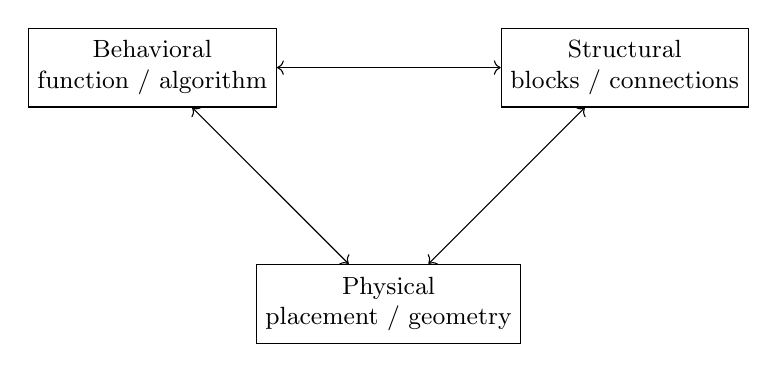
\begin{tikzpicture}[font=\small]
\node[draw,align=center,minimum width=3.1cm,minimum height=1cm] (b) at (-3,1.6) {Behavioral\\function / algorithm};
\node[draw,align=center,minimum width=3.1cm,minimum height=1cm] (s) at (3,1.6) {Structural\\blocks / connections};
\node[draw,align=center,minimum width=3.1cm,minimum height=1cm] (p) at (0,-1.4) {Physical\\placement / geometry};
\draw[<->] (b)--(s);\draw[<->] (b)--(p);\draw[<->] (s)--(p);
\end{tikzpicture}
\end{latin}
\caption{بازنمایی مفهومی رابطه سه دامنه، بر پایه بحث نمودار \lr{Y} کتاب
\cite{weste}. این شکل بازتولید هندسی خود نمودار \lr{Y} نیست؛
تبدیل دامنه‌ها در یک سطح مشخص را برجسته می‌کند.}
\label{fig:design-domains}
\end{figure}

\subsection{مثال بررسی رابط}
فرض کنید بلوکی \lr{MUX} هشت‌بیتی دارد و انتخابش با یک بیت \(S\) انجام می‌شود.
باید معلوم باشد \(S=0\) کدام ورودی را انتخاب می‌کند، هر ورودی چه زمانی معتبر است
و خروجی چه زمانی مصرف می‌شود. اتصال ورودی هفت‌بیتی به آن، یا برداشت معکوس از
معنای \(S\)، می‌تواند عملکرد را عوض کند؛ حتی اگر نام بلوک درست باشد.
در ادامه، همین انضباط را برای رابط پردازنده و حافظه به کار می‌بریم.

% !TeX root = booklet-01.tex
\section{مقدمات لازم برای مثال پردازنده \lr{MIPS}}
\subsection{پردازنده، حافظه، ثبات و دستور}
\lr{Processor} دستورها را از حافظه می‌خواند و طبق معنای آن‌ها داده‌ها و
حالت داخلی را تغییر می‌دهد. \lr{Memory} داده را در مکان‌های دارای آدرس نگه می‌دارد؛
آدرس، شماره مکان است و با محتوای آن مکان فرق دارد.
\lr{Register} محل کوچک ذخیره درون پردازنده و \lr{Register File}
مجموعه‌ای از این ثبات‌ها با مدار انتخاب و خواندن/نوشتن است.
این مقدمه برای خواندن بخش \secnum{۱.۷} کتاب لازم است \cite{weste}.

\lr{Instruction} یک الگوی بیت است که عملیات و عملوندها را مشخص می‌کند.
\lr{Program Counter (PC)} آدرس لازم برای خواندن جریان دستورها را نگه می‌دارد؛
در این طراحی، هنگام چهار \lr{Fetch} بایتی، به آدرس بایت بعدی پیش می‌رود.
\lr{Instruction Register (IR)} خود دستور خوانده‌شده را ذخیره می‌کند.
پس \lr{PC} آدرس است و \lr{IR} محتوا؛ جابه‌جا گرفتن این دو، مسیر داده را نامفهوم می‌کند.

دستور \code{add \$1, \$2, \$3} یعنی محتوای ثبات‌های دوم و سوم خوانده و
جمع در ثبات اول نوشته شود؛ اعداد نام ثبات‌اند، نه مقادیر داده.
اگر ثبات دوم ۵ و سوم ۷ داشته باشد، نتیجه ۱۲ است، نه جمع عددهای ۲ و ۳.
حروف \lr{Assembly} برای انسان خوانا هستند؛ سخت‌افزار کد دودویی متناظر را دریافت می‌کند.
\lr{Assembler} این کدگذاری را انجام می‌دهد؛ \lr{Compiler} زبان سطح بالا را
به نمایش پایین‌تر برنامه ترجمه می‌کند.

\subsection{عرض داده با عرض دستور یکسان نیست}
در زیرمجموعه کتاب، هشت ثبات عمومی هشت‌بیتی با نام‌های \code{\$0} تا \code{\$7}
و یک \lr{PC} هشت‌بیتی داریم؛ \code{\$0} همواره صفر است.
دستورها ۳۲ بیت و رابط داده حافظه هشت‌بیتی است
\cite[بخش \secnum{۱.۷.۱}]{weste}.
بنابراین ذخیره یک دستور در \lr{IR}، به چهار بایت هشت‌بیتی نیاز دارد:
\begin{equation}\label{eq:mips-fetch-width}
N_{\mathrm{bytes}}=\frac{32\ \mathrm{bits}}{8\ \mathrm{bits/byte}}=4\ \mathrm{bytes}.
\end{equation}
این نسبت، تعداد انتقال را می‌دهد؛ فرض شده هر چرخه یک بایت در دسترس است.
در طراحی دارای انتظار حافظه، تعداد چرخه می‌تواند بیشتر شود.

یک بیت دو حالت دارد؛ هشت بیت بدون علامت از صفر تا \(2^8-1=255\)
را نمایش می‌دهند. برای آدرس بایتی هشت‌بیتی، ۲۵۶ آدرس متمایز داریم.
اگر همه این فضا فقط دستورهای چهار‌بایتی باشد، حداکثر ۶۴ دستور جا می‌گیرد؛
ولی حافظه این مثال میان دستور و داده مشترک است و این تعداد ظرفیت آزاد واقعی برنامه را تضمین نمی‌کند.

برای نمایش منفی، قرارداد \lr{Two's Complement} را لازم داریم.
در هشت بیت، الگوی همه‌یک هم مقدار بدون علامت ۲۵۵ و هم مقدار علامت‌دار منفی یک
را می‌تواند نمایش دهد؛ تفسیر را عملیات تعیین می‌کند.
روش ساخت منفی یک از مثبت یک این است که بیت‌ها را مکمل و سپس یک اضافه کنیم:
\begin{latin}
\begin{verbatim}
 00000001   +1
 11111110   bitwise complement
 11111111   add one: -1 in signed 8-bit form
\end{verbatim}
\end{latin}
جمع هشت‌بیتی با نگه داشتن هشت بیت پایین، حساب پیمانه ۲۵۶ است؛
مثلاً الگوی ۲۵۵ به‌علاوه یک، هشت بیت پایین صفر و یک نقلی بیرونی می‌دهد.
این بیان حساب بیت‌هاست؛ پیاده‌سازی کامل استثناهای معماری \lr{MIPS32} را برای این مثال فرض نمی‌کنیم.

\section{مجموعه دستورها و کدگذاری}
\subsection{معنای ده دستور پشتیبانی‌شده}
کتاب دستورهای \code{ADD}، \code{SUB}، \code{AND}، \code{OR}، \code{SLT}،
\code{ADDI}، \code{BEQ}، \code{J}، \code{LB} و \code{SB} را معرفی می‌کند
\cite[جدول \secnum{۱.۷}]{weste}.
در جدول \ref{tab:mips-isa}، \(R_a,R_b,R_d\) محتوای ثبات، \(M[a]\)
بایت حافظه در آدرس \(a\) و \(\mathrm{imm}\) مقدار ثابت داخل دستور است.
پیکان \(\leftarrow\) یعنی نوشتن مقدار جدید و معادله تساوی دو مقدار هم‌زمان نیست.

\begin{table}[ht]
\centering
\caption{معنای دستورهای زیرمجموعه آموزشی؛ برای تغییر \lr{PC}، جزئیات متن را نیز بخوانید.}
\label{tab:mips-isa}
\begin{tabularx}{\textwidth}{lXl}
\toprule
دستور & اثر اصلی & \code{op}\\
\midrule
\code{ADD}&\(R_d\leftarrow R_a+R_b\)&\code{000000}\\
\code{SUB}&\(R_d\leftarrow R_a-R_b\)&\code{000000}\\
\code{AND}&عمل \lr{AND} بیت‌به‌بیت دو ثبات&\code{000000}\\
\code{OR}&عمل \lr{OR} بیت‌به‌بیت دو ثبات&\code{000000}\\
\code{SLT}&نوشتن یک در مقصد اگر شرط کمتر بودن برقرار باشد، وگرنه صفر&\code{000000}\\
\code{ADDI}&جمع ثبات با ثابت \lr{Immediate} و نوشتن در ثبات مقصد&\code{001000}\\
\code{BEQ}&اگر دو ثبات برابر باشند، انتقال به آدرس نسبی شاخه&\code{000100}\\
\code{J}&انتقال به مقصد پرش کدگذاری‌شده&\code{000010}\\
\code{LB}&\(R_b\leftarrow M[R_a+\mathrm{imm}]\)؛ خواندن یک بایت&\code{100000}\\
\code{SB}&\(M[R_a+\mathrm{imm}]\leftarrow R_b\)؛ نوشتن یک بایت&\code{101000}\\
\bottomrule
\end{tabularx}
\end{table}
در \code{LB} و \code{SB}، دو جمع متفاوت نداریم؛ ابتدا آدرس موثر با جمع
پایه و جابه‌جایی ساخته و سپس حافظه با همان آدرس استفاده می‌شود.
\code{AND} و \code{OR} روی هر جفت بیت متناظر مستقل عمل می‌کنند.
تفسیر علامت‌دار و رفتار سرریز در مقایسه و حساب باید در مشخصات پیاده‌سازی دقیق روشن باشد؛
مثال‌های عددی مقایسه این جزوه در محدوده بدون ابهام سرریز انتخاب می‌شوند.

\subsection{قالب‌های \lr{R}، \lr{I} و \lr{J}}
در هر سه قالب، شش بیت بالایی \code{op} هستند. قالب \lr{R} پنج فیلد دیگر دارد:
\code{rs}، \code{rt}، \code{rd}، \code{shamt} و \code{funct}.
سه فیلد ثبات هرکدام پنج بیت‌اند؛ در زیرمجموعه هشت‌ثباتی، فقط نام‌های مجاز
صفر تا هفت استفاده می‌شوند، هرچند محل کدگذاری پنج‌بیتی حفظ شده است.
فیلد پنج‌بیتی \code{shamt} در دستورهای \lr{R} مورد بحث صفر است.
قالب \lr{I} دو فیلد ثبات و ثابت ۱۶بیتی و قالب \lr{J} مقصد ۲۶بیتی دارد
\cite[شکل \secnum{۱.۴۹}]{weste}.

شمارش طول فیلدها، یک کنترل ساده بر کدگذاری است:
\begin{align}
\mathrm{R}:&\quad 6+5+5+5+5+6=32,\notag\\
\mathrm{I}:&\quad 6+5+5+16=32,\notag\\
\mathrm{J}:&\quad 6+26=32.
\label{eq:mips-fields}
\end{align}
دستورهای \lr{R} این مثال همگی \code{op=000000} دارند و \code{funct}
عملیات را جدا می‌کند؛ مثلاً \code{100000} برای جمع و \code{100010} برای تفریق.
قالب ۳۲بیتی را نباید به دلیل داده هشت‌بیتی به قالب کوتاه‌تر تبدیل کرد.

\subsection{مثال خواندن بیت‌ها و \lr{Hexadecimal}}
در مبنای شانزده، هر رقم چهار بیت را نمایش می‌دهد؛ پس ۳۲ بیت با هشت رقم
نمایش داده می‌شود. حروف \code{a} تا \code{f} به‌ترتیب مقادیر ده تا پانزده‌اند.
مثلاً \code{1111} برابر \code{f} است؛ این حروف بخشی از عددند، نه نام متغیر.

دستور \code{addi \$3, \$0, 8} به‌ترتیب فیلدهای زیر را دارد:
\begin{latin}
\begin{verbatim}
op     rs    rt    immediate
001000 00000 00011 0000000000001000
0010 0000 0000 0011 0000 0000 0000 1000
   2    0    0    3    0    0    0    8
\end{verbatim}
\end{latin}
پس کد \lr{Hex} برابر \code{20030008} است. مقدار ۸ در ثبات سوم نوشته می‌شود،
چون ثبات صفر مقدار صفر می‌دهد. در \code{addi \$5, \$0, -1}، ثابت ۱۶بیتی
\code{ffff} است؛ هشت بیت پایین آن در مسیر داده هشت‌بیتی، الگوی \code{ff} را می‌دهد.
این کوچک شدن مسیر داده، فیلد ذخیره‌شده ۱۶بیتی داخل دستور را تغییر نمی‌دهد.

\subsection{آدرس شاخه و پرش را با واحد بایت بخوانیم}
دستورها چهار بایت‌اند؛ مقصد نسبی شاخه در واحد کلمه دستور کدگذاری می‌شود.
پس باید جابه‌جایی در چهار ضرب شود؛ این کار با دو بیت شیفت چپ متناظر است.
اگر آدرس شروع دستور \(P\) باشد، پس از \lr{Fetch} چهار بایت، \lr{PC} به
\(P+4\) رسیده است؛ در صورت برابری دو ثبات، مقصد شاخه در این مثال برابر است با:
\begin{equation}\label{eq:mips-branch}
PC_{\mathrm{target}}=(P+4+4\,\mathrm{imm})\bmod256.
\end{equation}
نماد \(\bmod256\) یعنی نگه داشتن باقیمانده در بازه صفر تا ۲۵۵،
متناسب با \lr{PC} هشت‌بیتی. برای \(\mathrm{imm}\) منفی،
تفسیر علامت‌دار جابه‌جایی لازم است؛ محاسبه پیمانه‌ای نتیجه بیت‌های پایین را مشخص می‌کند.
استفاده از \(P\) به‌جای \(P+4\) یک دستور خطای مقصد ایجاد می‌کند.

در برنامه کتاب، شاخه در آدرس ۱۲ و برچسب پایان در آدرس ۳۲ است؛
پس مقدار جابه‌جایی دستور شاخه چنین محاسبه می‌شود.
\[
 \mathrm{imm}=\frac{32-16}{4}=4.
\]
برای پرش به آدرس ۱۲، فیلد مقصد \(12/4=3\) است؛
سخت‌افزار با شیفت چپ دو بیت، آن را به آدرس بایتی برمی‌گرداند.
قاعده ترکیب بیت‌های بالایی مقصد در معماری کامل ۳۲بیتی را نباید بدون توجه
به \lr{PC} هشت‌بیتی این مدل به شکل مثال تحمیل کرد
\cite[جدول \secnum{۱.۷}، شکل‌های \secnum{۱.۵۲} و \secnum{۱.۵۳}]{weste}.

\section{مثال \lr{Fibonacci}: از برنامه تا کد ماشین}
\subsection{مقادیر اولیه و ترتیب به‌روزرسانی}
مثال \secnum{۱.۴} کتاب تابع بازگشتی را با
\(f_{-1}=-1\)، \(f_0=1\) و \(f_n=f_{n-1}+f_{n-2}\) برای \(n>0\)
تعریف می‌کند. این مقادیر اولیه با قرارداد رایج \(F_0=0,F_1=1\) یکسان نیستند؛
پس نام \lr{Fibonacci} به‌تنهایی پاسخ عددی را تعیین نمی‌کند
\cite[شکل \secnum{۱.۵۰}]{weste}.
در برنامه، \code{f1} ابتدا یک و \code{f2} منفی یک است و حلقه هشت بار اجرا می‌شود:
\begin{latin}
\begin{verbatim}
f1 = f1 + f2;
f2 = f1 - f2;
n  = n - 1;
\end{verbatim}
\end{latin}
این سه خط نرم‌افزاری به‌ترتیب اجرا می‌شوند. اگر مقادیر قدیمی را \(a,b\)
بنامیم، بعد از خط اول \(f1=a+b\) و بعد از خط دوم
\(f2=(a+b)-b=a\) می‌شود. بنابراین زوج به \((a+b,a)\) تبدیل می‌شود.
اگر در خط دوم به اشتباه از \code{f1} قدیمی استفاده کنیم، الگوریتم دیگری خواهیم داشت.

جدول \ref{tab:mips-fib} نتیجه اجرای مستقل همین ترتیب را نشان می‌دهد؛
در این ورودی، مقادیر نتیجه از محدوده علامت‌دار هشت‌بیتی خارج نمی‌شوند.
\begin{table}[ht]
\centering
\caption{ردگیری آموزشی حلقه با مقادیر اولیه دقیق کتاب؛ ستون‌ها مقدار پس از تکرار را نشان می‌دهند.}
\label{tab:mips-fib}
\begin{tabular}{cccc}
\toprule
تعداد تکرار اجراشده & شمارنده باقی‌مانده & \code{f1} & \code{f2}\\
\midrule
۰&۸&۱&\(-1\)\\
۱&۷&۰&۱\\
۲&۶&۱&۰\\
۳&۵&۱&۱\\
۴&۴&۲&۱\\
۵&۳&۳&۲\\
۶&۲&۵&۳\\
۷&۱&۸&۵\\
۸&۰&۱۳&۸\\
\bottomrule
\end{tabular}
\end{table}
پس مقدار ذخیره‌شده نهایی ۱۳ است. برنامه صرفاً نام دنباله را به کار نبرده،
بلکه قرارداد دقیق اولیه و عملیات ترتیب‌دار دارد.

\subsection{خواندن برنامه \lr{Assembly}}
در شکل \secnum{۱.۵۱} کتاب، ثبات سوم شمارنده، چهارم \code{f1} و پنجم
\code{f2} است. برچسب‌ها نشانی‌اند و خودشان دستور اجرایی نیستند.
برنامه زیر همان دستورها را با توضیح انگلیسی کوتاه بازنویسی می‌کند:
\begin{latin}
\small
\begin{verbatim}
fib:  addi $3, $0, 8     # n = 8
      addi $4, $0, 1     # f1 = 1
      addi $5, $0, -1    # f2 = -1
loop: beq  $3, $0, end   # exit when n == 0
      add  $4, $4, $5    # update f1 first
      sub  $5, $4, $5    # use the new f1
      addi $3, $3, -1    # decrement n
      j    loop
end:  sb   $4, 255($0)   # write result to byte address 255
\end{verbatim}
\end{latin}
وقتی شمارنده صفر شود، \code{beq} به \code{end} می‌رود و یک بایت نتیجه را
در آدرس ۲۵۵ می‌نویسد. صفر بودن \code{\$0} آدرس موثر \(0+255\) را می‌دهد.
این برنامه دستور \code{HALT} ندارد؛ مشاهده نوشتن نتیجه، به معنی توقف ذاتی پردازنده نیست.

\subsection{تطبیق همه کدهای ماشین مثال}
جدول \ref{tab:mips-machine} کدهای شکل \secnum{۱.۵۲} کتاب را با آدرس بایتی
دستورها کنار هم می‌گذارد. فرض این جدول، شروع برنامه از آدرس صفر است.
\begin{table}[ht]
\centering
\caption{کدهای ماشین برنامه کتاب؛ رشته‌های کد و شناسه‌ها با ارقام \lr{Latin} اصلی حفظ شده‌اند.}
\label{tab:mips-machine}
\begin{tabular}{cll}
\toprule
آدرس بایتی & دستور & کد \lr{Hex}\\
\midrule
۰&\code{addi \$3, \$0, 8}&\code{20030008}\\
۴&\code{addi \$4, \$0, 1}&\code{20040001}\\
۸&\code{addi \$5, \$0, -1}&\code{2005ffff}\\
۱۲&\code{beq \$3, \$0, end}&\code{10600004}\\
۱۶&\code{add \$4, \$4, \$5}&\code{00852020}\\
۲۰&\code{sub \$5, \$4, \$5}&\code{00852822}\\
۲۴&\code{addi \$3, \$3, -1}&\code{2063ffff}\\
۲۸&\code{j loop}&\code{08000003}\\
۳۲&\code{sb \$4, 255(\$0)}&\code{a00400ff}\\
\bottomrule
\end{tabular}
\end{table}
برای کنترل مستقل، می‌توان هر کد را به فیلدها شکست؛ مثلاً \code{00852020}
ثبات‌های منبع چهار و پنج، مقصد چهار و \code{funct=100000} را می‌دهد.
برای شاخه نیز آدرس ۱۲، \lr{PC} بعد از \lr{Fetch} برابر ۱۶ و جابه‌جایی چهار کلمه
با مقصد ۳۲ سازگار است.

% !TeX root = booklet-01.tex
\section{اجرای چندچرخه‌ای و مسیر داده}
\label{sec:mips-micro}
\subsection{چرا \lr{Multicycle}؟}
در پیاده‌سازی \lr{Multicycle}، یک دستور در چند چرخه اجرا می‌شود و یک منبع
می‌تواند در چرخه‌های مختلف چند کار انجام دهد. در این مثال، همان \lr{ALU}
ابتدا \lr{PC} را افزایش می‌دهد، سپس آدرس یا نتیجه حسابی را محاسبه می‌کند.
ثبات‌های میانی، نتیجه را تا زمان مصرف نگه می‌دارند
\cite[بخش \secnum{۱.۷.۲}]{weste}.
صرف چندچرخه‌ای بودن، اجرای هم‌زمان چند دستور یا \lr{Pipeline} را ثابت نمی‌کند؛
این کنترل‌کننده یک دستور را به‌ترتیب مراحلش جلو می‌برد.

\lr{Datapath} شامل مسیرهای داده، \lr{MUX}ها، ثبات‌ها، \lr{Register File}
و \lr{ALU} است. \lr{Controller} با دیدن نوع دستور، حالت جاری و پرچم‌هایی
مثل \code{Zero}، انتخاب مسیر و اجازه نوشتن را مشخص می‌کند.
شکل \ref{fig:mips-overview} جداسازی این دو مسئولیت را نشان می‌دهد.

\begin{figure}[ht]
\centering
\begin{latin}
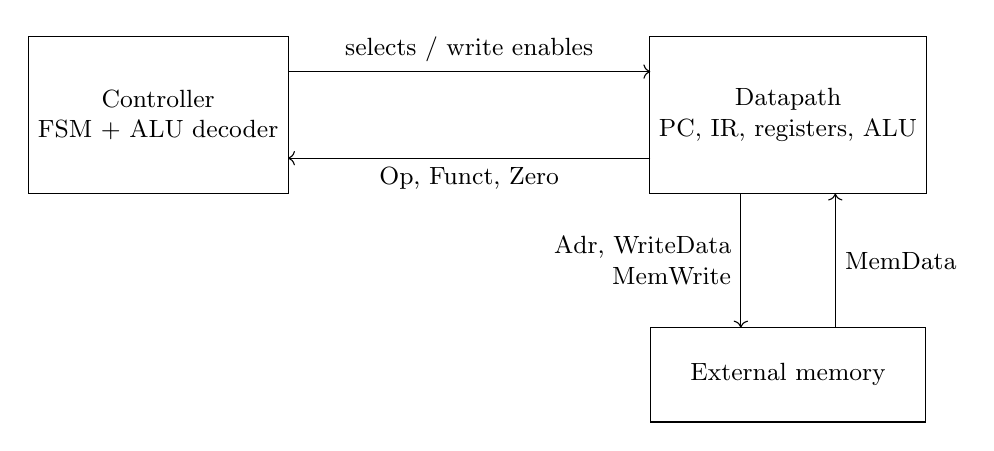
\begin{tikzpicture}[font=\small]
\node[draw,minimum width=3.3cm,minimum height=2cm,align=center] (c) at (0,0) {Controller\\FSM + ALU decoder};
\node[draw,minimum width=3.5cm,minimum height=2cm,align=center] (d) at (8,0) {Datapath\\PC, IR, registers, ALU};
\draw[->] (1.65,0.55)--node[above] {selects / write enables}(6.25,0.55);
\draw[->] (6.25,-0.55)--node[below] {Op, Funct, Zero}(1.65,-0.55);
\node[draw,minimum width=3.5cm,minimum height=1.2cm] (m) at (8,-3.3) {External memory};
\draw[->] (7.4,-1)--node[left,align=right] {Adr, WriteData\\MemWrite}(7.4,-2.7);
\draw[->] (8.6,-2.7)--node[right] {MemData}(8.6,-1);
\end{tikzpicture}
\end{latin}
\caption{نمای فشرده آموزشی مسیر داده و کنترل، بر پایه شکل‌های \secnum{۱.۵۳}
و \secnum{۱.۵۶} کتاب \cite{weste}. این شکل همه سیم‌ها و \lr{MUX}های شکل اصلی را رسم نمی‌کند؛
انتخاب‌های آن‌ها در جدول \ref{tab:mips-selects} آمده‌اند.}
\label{fig:mips-overview}
\end{figure}

\subsection{نقش ثبات‌های میانی}
\lr{IR} دستور ۳۲بیتی را نگه می‌دارد؛ ثبات \code{Data} بایت خوانده‌شده حافظه
را برای نوشتن بعدی در ثبات مقصد حفظ می‌کند.
ثبات‌های \code{A} و \code{B} دو داده خوانده‌شده از \lr{Register File} را
در اختیار \lr{ALU} می‌گذارند. \code{ALUOut} نیز نتیجه مرحله قبل، مانند
آدرس موثر یا نتیجه حسابی را نگه می‌دارد.
بنابراین \code{ALUResult}، خروجی محاسبه جاری و \code{ALUOut}، مقدار ثبت‌شده‌اند؛
هم‌نام یا هم‌زمان بودن مقدارشان را نباید فرض کرد.

\lr{MUX} ورودی اول \lr{ALU} بین \lr{PC} و \code{A} انتخاب می‌کند؛
ورودی دوم می‌تواند \code{B}، ثابت یک، بخش ثابت دستور یا ثابت ضرب‌شده در چهار باشد.
\code{PCEn} اجازه نوشتن \lr{PC} است و در مدل شکل کتاب از رابطه زیر می‌آید:
\begin{equation}\label{eq:mips-pcen}
\mathrm{PCEn}=\mathrm{PCWrite}+(\mathrm{Branch}\cdot\mathrm{Zero}).
\end{equation}
علامت جمع اینجا \lr{OR} منطقی است. \code{PCWrite} نوشتن بی‌قید به برابری
و \code{Branch} همراه \code{Zero} نوشتن مشروط را فعال می‌کند.
در \code{BEQ}، تفریق دو عملوند اگر صفر شود، برابری را نشان می‌دهد.

\subsection{معنای دقیق انتخاب‌گرها}
جدول \ref{tab:mips-selects} قرارداد شکل \secnum{۱.۵۳} کتاب را باز می‌کند.
اعداد انتخاب، کدهای همان طراحی‌اند و استاندارد همگانی سیگنال‌های هم‌نام نیستند.
\begin{table}[ht]
\centering
\caption{انتخاب مسیرها در \lr{Datapath} آموزشی کتاب}
\label{tab:mips-selects}
\begin{tabularx}{\textwidth}{lX}
\toprule
کنترل & انتخاب در شکل کتاب\\
\midrule
\code{IorD}&\code{0}: آدرس حافظه از \lr{PC}؛ \code{1}: از \code{ALUOut}\\
\code{ALUSrcA}&\code{0}: \lr{PC}؛ \code{1}: ثبات موقت \code{A}\\
\code{ALUSrcB}&\code{00}: \code{B}؛ \code{01}: یک؛ \code{10}: ثابت داده؛ \code{11}: ثابت ضرب‌شده در چهار\\
\code{PCSrc}&\code{00}: \code{ALUResult}؛ \code{01}: \code{ALUOut}؛ \code{10}: مقصد پرش\\
\code{RegDst}&\code{0}: فیلد \code{rt}؛ \code{1}: فیلد \code{rd}\\
\code{MemtoReg}&\code{0}: \code{ALUOut}؛ \code{1}: ثبات \code{Data}\\
\code{IRWrite[3:0]}&چهار اجازه نوشتن مستقل برای چهار بایت \lr{IR}\\
\code{RegWrite}&اجازه نوشتن در \lr{Register File}\\
\code{MemWrite}&اجازه نوشتن حافظه بیرونی\\
\bottomrule
\end{tabularx}
\end{table}
در آدرس‌های هشت‌بیتی، خروجی محاسبات آدرس به هشت بیت محدود است.
برای داده، ثابت از بیت‌های پایین دستور وارد مسیر هشت‌بیتی می‌شود؛
برای شاخه، مسیر شیفت چپ دو بیت جداگانه در شکل مشخص است.
وجود نام \code{MemtoReg} به معنی انتخاب همیشگی حافظه نیست؛ مقدار کنترل مسیر را تعیین می‌کند.

\subsection{چهار \lr{Fetch} و ترتیب بایت‌های \lr{IR}}
حالت‌های صفر تا سه کنترل‌کننده، هرکدام یک بایت را از آدرس \lr{PC} می‌خوانند
و در یک بخش \lr{IR} می‌نویسند. در همان چرخه، \lr{ALU} با انتخاب
\code{ALUSrcA=0} و \code{ALUSrcB=01}، مقدار \(PC+1\) را تولید می‌کند.
\code{PCWrite=1} و \code{PCSrc=00} اجازه ثبت آن را می‌دهند
\cite[مثال \secnum{۱.۵}]{weste}.

در حالت اول، \code{IRWrite0} بایت کم‌ارزش را ثبت می‌کند؛ سه حالت بعدی
به‌ترتیب بایت‌های دیگر را می‌نویسند. برای کد \code{20030008} در حافظه بایتی،
ترتیب \code{08, 00, 03, 20} در آدرس‌های پیاپی با این قرارداد سازگار است.
پس کد نمایش‌داده‌شده ۳۲بیتی با ترتیب نمایش بایت‌های حافظه یکی نیست.
بعد از چهار انتقال، دستور کامل و \lr{PC} آماده نشانی دستور بعدی است.

متن مثال کتاب نام \code{MemRead} را نیز هنگام توصیف خواندن می‌آورد؛
ولی رابط نهایی جدول \secnum{۱.۹} پایه مستقلی با این نام ندارد.
در این جزوه خواندن را در چارچوب حافظه ساده همان شکل تفسیر می‌کنیم و
پایه جدیدی به رابط اضافه نمی‌کنیم. برای حافظه واقعی با پروتکل یا زمان انتظار،
قرارداد خواندن باید جداگانه مشخص شود.

\section{ماشین حالت و اجرای دستورها}
\subsection{مفهوم \lr{FSM} و جدول حالت‌های کتاب}
\lr{Finite State Machine (FSM)} مجموعه محدودی از حالت‌ها، قانون انتقال
و خروجی‌های کنترلی دارد. حالت، مرحله اجرای فعلی را نگه می‌دارد؛
\code{op} مشخص می‌کند پس از \lr{Decode} به کدام مسیر برویم.
جدول \ref{tab:mips-fsm} حالت‌های شکل \secnum{۱.۵۴} را خلاصه می‌کند
\cite{weste}.

\begin{table}[ht]
\centering
\caption{حالت‌های رسم‌شده کنترل‌کننده کتاب؛ شماره‌ها شناسه حالت‌اند، نه شماره چرخه همه دستورها.}
\label{tab:mips-fsm}
\begin{tabularx}{\textwidth}{cXX}
\toprule
حالت & عمل اصلی & مسیر بعدی\\
\midrule
۰، ۱، ۲، ۳&\lr{Fetch} چهار بایت و افزایش بایتی \lr{PC}&به‌ترتیب تا حالت ۴\\
۴&\lr{Decode}، خواندن دو ثبات و محاسبه مقصد احتمالی شاخه&با توجه به \code{op} به ۵، ۹، ۱۱ یا ۱۲\\
۵&محاسبه آدرس موثر برای \code{LB/SB}&برای \code{LB} به ۶؛ برای \code{SB} به ۸\\
۶&خواندن بایت حافظه و ثبت در \code{Data}&۷\\
۷&نوشتن داده حافظه در ثبات مقصد&۰\\
۸&نوشتن بایت \code{B} در حافظه&۰\\
۹&اجرای عمل \lr{R-type} و ثبت نتیجه&۱۰\\
۱۰&نوشتن \code{ALUOut} در ثبات مقصد&۰\\
۱۱&مقایسه برای \code{BEQ} و تغییر مشروط \lr{PC}&۰\\
۱۲&ثبت مقصد \code{J} در \lr{PC}&۰\\
\bottomrule
\end{tabularx}
\end{table}

حالت‌های اجرای \code{ADDI} در شکل کتاب رسم نشده‌اند و به‌عنوان تمرین
خواننده باقی گذاشته شده‌اند. بنابراین جدول را کنترل‌کننده کامل همه ده دستور
اعلام نمی‌کنیم. مسیر \code{ADDI} برای اجرای برنامه لازم است؛ از نظر رفتاری
باید \code{A} را با ثابت جمع و نتیجه را در \code{rt} ثبت کند، اما این توصیف
جای پیاده‌سازی و تایید حالت‌های اضافه را نمی‌گیرد.

\subsection{ردگیری کامل \code{SUB}}
برای \code{sub \$5, \$4, \$5}، چهار \lr{Fetch} ابتدا \lr{IR} را کامل می‌کنند.
در حالت ۴، فیلدهای \code{rs} و \code{rt} ثبات‌های چهار و پنج را می‌خوانند
و در \code{A} و \code{B} قرار می‌دهند.
محاسبه جانبی مقصد شاخه در همین حالت برای این دستور مصرف نمی‌شود.

در حالت ۹، \code{ALUSrcA=1} و \code{ALUSrcB=00} دو داده را به
\lr{ALU} می‌فرستند. \code{ALUOp=10} یعنی نوع عمل از \code{funct}
تعیین شود؛ برای \code{funct=100010}، کنترل \code{110} تفریق را انتخاب می‌کند.
نتیجه در \code{ALUOut} ثبت می‌شود.
در حالت ۱۰، \code{RegDst=1} مقصد \code{rd}،
\code{MemtoReg=0} داده \code{ALUOut} و \code{RegWrite=1} اجازه نوشتن را
انتخاب می‌کنند؛ سپس کنترل به \lr{Fetch} بعدی برمی‌گردد
\cite[مثال \secnum{۱.۵}، صفحات چاپی ۳۷ و ۳۸]{weste}.

پس این \lr{R-type} در مدل بدون انتظار حافظه، چهار \lr{Fetch}، یک \lr{Decode}،
یک \lr{Execute} و یک \lr{Write-back}، یعنی هفت چرخه دارد.
عبارت «سه مرحله برای جمع یا تفریق» پس از \lr{Fetch}، نباید با سه چرخه برای کل دستور اشتباه شود.

\subsection{چرا شاخه به نتیجه ثبت‌شده قبلی نیاز دارد؟}
در حالت ۴، \lr{ALU} از \lr{PC} بعد از \lr{Fetch} و ثابت ضرب‌شده در چهار،
مقصد احتمالی را می‌سازد و در \code{ALUOut} قرار می‌دهد.
در حالت ۱۱، همان \lr{ALU} برای تفریق \code{A-B} استفاده می‌شود تا
\code{Zero} به دست آید؛ مقصد از \code{ALUOut} قبلی انتخاب می‌شود، نه خروجی
تفریق جاری. این استفاده دوباره از منبع، دلیل اهمیت ثبات موقت است.

اگر داده‌ها برابر باشند، \code{Branch=1} و \code{Zero=1} طبق رابطه
\eqref{eq:mips-pcen}، \lr{PC} را با مقصد شاخه به‌روزرسانی می‌کنند؛
اگر برابر نباشند، \lr{PC} همان آدرس بعد از \lr{Fetch} را نگه می‌دارد.
در نمونه هشت‌بیتی، تفریق صفر دقیقاً برابری دو الگوی هشت‌بیتی را نشان می‌دهد.

\subsection{تفاوت مسیر \code{LB} و \code{SB}}
هر دو پس از \lr{Decode} در حالت ۵، آدرس \(R_a+\mathrm{imm}\) را
در \code{ALUOut} ثبت می‌کنند. با \code{IorD=1}، آدرس حافظه از این ثبات می‌آید.
\code{LB} در حالت ۶ بایت را می‌خواند و در حالت ۷ با
\code{RegDst=0, MemtoReg=1, RegWrite=1} در \code{rt} می‌نویسد.
\code{SB} در حالت ۸ داده \code{B} را با \code{MemWrite=1} به حافظه می‌دهد.
بنابراین \code{LB} هشت و \code{SB} هفت چرخه در نمودار رسم‌شده نیاز دارند.
\code{BEQ} و \code{J} هرکدام با چهار \lr{Fetch}، \lr{Decode} و یک مرحله نهایی، شش چرخه دارند.

\subsection{\lr{Decode} عمل \lr{ALU} را با حالت اجرا یکی نگیریم}
جدول \ref{tab:mips-aludec} از جدول \secnum{۱.۸} کتاب گرفته شده است.
\code{x} یعنی مقدار آن فیلد برای همان تصمیم استفاده نمی‌شود؛ به معنی
ایجاد حالت ناشناخته در همه خروجی‌ها نیست.
\begin{table}[ht]
\centering
\caption{تفکیک \code{ALUOp} تولیدشده توسط \lr{FSM} از \code{ALUControl} محلی}
\label{tab:mips-aludec}
\begin{tabular}{llll}
\toprule
\code{ALUOp}&\code{funct}&\code{ALUControl}&عمل\\
\midrule
\code{00}&\code{x}&\code{010}&\code{ADD}\\
\code{01}&\code{x}&\code{110}&\code{SUB}\\
\code{10}&\code{100000}&\code{010}&\code{ADD}\\
\code{10}&\code{100010}&\code{110}&\code{SUB}\\
\code{10}&\code{100100}&\code{000}&\code{AND}\\
\code{10}&\code{100101}&\code{001}&\code{OR}\\
\code{10}&\code{101010}&\code{111}&\code{SLT}\\
\code{11}&\code{x}&\code{x}&تعریف‌نشده در جدول\\
\bottomrule
\end{tabular}
\end{table}
خود \lr{FSM} حالت‌دار است، ولی \lr{ALU Decoder} می‌تواند یک مدار
\lr{Combinational} از کد عمل و \code{funct} باشد.
یکسان بودن \lr{ALUControl} برای جمعِ \lr{Fetch} و جمعِ دستور،
به معنی یکسان بودن بقیه انتخاب‌ها و مقصد ثبت نیست.

% !TeX root = booklet-01.tex
\section{از رابط پردازنده تا \lr{Logic Design}}
\subsection{رابط سطح بالا را پیش از طراحی داخل مشخص کنیم}
رابط جدول \secnum{۱.۹} کتاب، ورودی‌های \code{ph1}، \code{ph2}،
\code{reset} و \code{MemData[7:0]} و خروجی‌های \code{MemWrite}،
\code{Adr[7:0]} و \code{WriteData[7:0]} را دارد
\cite[بخش \secnum{۱.۸.۱}]{weste}.
بازه \code{[7:0]} یعنی هشت بیت از شماره هفت تا صفر؛ تفریق هفت از صفر نیست.
\code{MemWrite} یک سیگنال کنترلی تک‌بیتی است و دو باس داده هرکدام هشت بیت‌اند.

دو ورودی ساعت، دو فاز غیرهم‌پوشان طراحی فیزیکی را بیان می‌کنند؛
نمای \code{CLK} در شکل کلی \lr{Microarchitecture} سطح انتزاع ساده‌تری است.
\code{reset} در متن کتاب \lr{PC} را صفر و کنترل‌کننده را به حالت آغازین می‌برد؛
از این جمله نباید صفرشدن تمام ثبات‌های داده را نتیجه گرفت.

در خواندن، پردازنده آدرس می‌دهد و حافظه \code{MemData} را برمی‌گرداند؛
در نوشتن، آدرس و \code{WriteData} همراه اجازه نوشتن ارائه می‌شوند.
کتاب در این مثال مسیر خواندن و نوشتن داده را جدا نگه می‌دارد.
ترکیب آن‌ها در باس دوطرفه ممکن است، ولی به کنترل جهت و جلوگیری از
راه‌اندازی متضاد نیاز دارد و تغییر ساده نام سیم نیست.
رابط حافظه دارای \lr{Handshake} یا چرخه انتظار، خارج از قرارداد ساده این مثال است.

\subsection{\lr{Wordslice}، \lr{Bitslice} و \lr{Zipper}}
در \lr{Wordslice}، یک واحد چندبیتی کامل مانند \lr{MUX} هشت‌بیتی یا ثبات
هشت‌بیتی را یک ستون می‌بینیم. در \lr{Bitslice}، یک ردیف شامل یک بیت
از هر واحد و اتصال‌های همان بیت است
\cite[بخش \secnum{۱.۸.۲} و شکل \secnum{۱.۵۷}]{weste}.
این دو، دو روش نگاه به سازمان فیزیکی و منطقی مسیر داده‌اند؛
یکی به معنی «هشت مدار متفاوت» و دیگری به معنی «بدون سیم بین بیت‌ها» نیست.

برای یک \lr{MUX} هشت‌بیتی، هشت \lr{MUX} تک‌بیتی داریم که همگی یک
انتخاب مشترک می‌گیرند. مدار بافر و تولید مکمل انتخاب را می‌توان در ناحیه مشترکی
قرار داد؛ کتاب به این ناحیه \lr{Zipper} می‌گوید.
این کار می‌تواند از تکرار هشت مدار تولید مکمل جلوگیری کند،
ولی طول سیم و بار مشترک باید بررسی شود. جای میانی یا کناری این ناحیه، تصمیم فیزیکی است.

در جمع‌کننده، \lr{Carry} از یک بیت به بیت دیگر می‌رود؛
در تشخیص صفر، خروجی بیت‌ها باید با هم ترکیب شوند.
پس همه اتصال‌ها صرفاً محلی و همه \lr{Bitslice}ها الزاماً مستقل و یکسان نیستند.
در همین مثال، کتاب \lr{Datapath} منظم را مناسب طراحی تکرارشونده و کنترل‌کننده
کم‌قاعده‌تر را مناسب توصیف انتزاعی و ابزار خودکار معرفی می‌کند.

\subsection{سلسله‌مراتب باید قابل ردیابی بماند}
شکل \ref{fig:logic-hierarchy} بخشی از سلسله‌مراتب کتاب را فشرده بازنمایی می‌کند.
\lr{Leaf Cell} پایین‌ترین بلوک در سطحی است که فعلاً به جزئیات آن وارد نمی‌شویم؛
ممکن است در سطح مدار خودش از چند ترانزیستور تشکیل شده باشد.

\begin{figure}[ht]
\centering
\begin{latin}
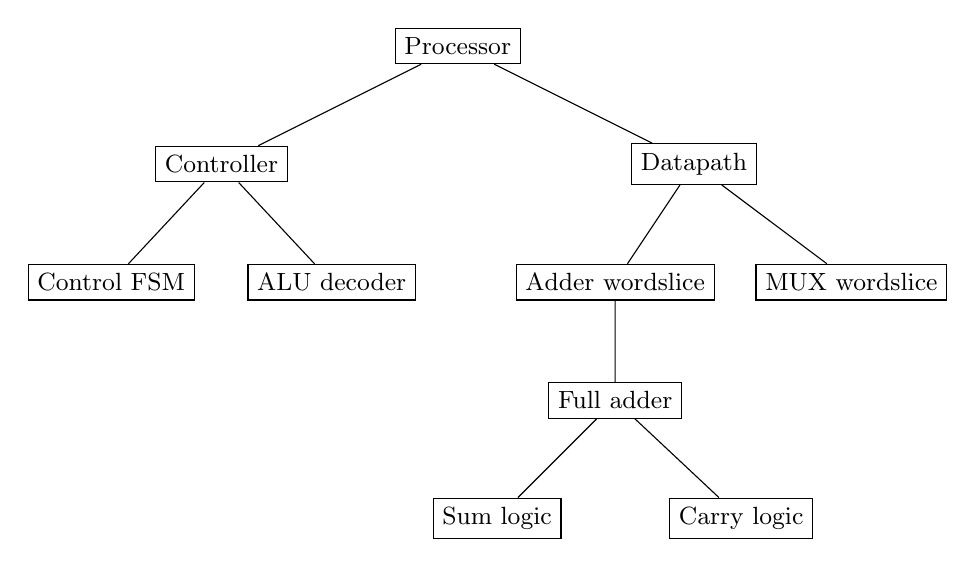
\begin{tikzpicture}[font=\small]
\node[draw] (top) at (0,3) {Processor};
\node[draw] (ctrl) at (-3,1.5) {Controller};
\node[draw] (data) at (3,1.5) {Datapath};
\node[draw,align=center] (fsm) at (-4.4,0) {Control FSM};
\node[draw,align=center] (dec) at (-1.6,0) {ALU decoder};
\node[draw] (add) at (2,0) {Adder wordslice};
\node[draw] (mux) at (5,0) {MUX wordslice};
\node[draw] (fa) at (2,-1.5) {Full adder};
\draw (top)--(ctrl) (top)--(data) (ctrl)--(fsm) (ctrl)--(dec);
\draw (data)--(add) (data)--(mux) (add)--(fa);
\node[draw] (sum) at (0.5,-3) {Sum logic};
\node[draw] (carry) at (3.6,-3) {Carry logic};
\draw (fa)--(sum) (fa)--(carry);
\end{tikzpicture}
\end{latin}
\caption{سلسله‌مراتب آموزشی فشرده بر پایه شکل \secnum{۱.۵۸} کتاب \cite{weste}؛
این شاخه‌ها تمام بلوک‌های پردازنده را فهرست نمی‌کنند.}
\label{fig:logic-hierarchy}
\end{figure}

سلسله‌مراتب منطقی، مداری و فیزیکی الزاماً یکسان نیست، اما تفاوت زیاد آن‌ها
تطبیق و \lr{Verification} را دشوار می‌کند.
مثلاً حافظه در نمای بالا یک بلوک است و در سطح مدار، آرایه و \lr{Decode} و مسیرهای
خواندن دارد. باید معلوم باشد هر بلوک در نمای دیگر کجا و چگونه پیاده شده است
\cite[بخش \secnum{۱.۸.۳}]{weste}.

\section{خواندن مقدماتی \lr{HDL}}
\subsection{توصیف سخت‌افزار با برنامه ترتیبی یکسان نیست}
\lr{Hardware Description Language (HDL)} مانند \lr{Verilog}،
\lr{SystemVerilog} یا \lr{VHDL} برای توصیف مدار به کار می‌رود.
دو سبک کلی، \lr{Structural} برای نمونه‌سازی و اتصال بلوک‌ها و
\lr{Behavioral} برای بیان رفتار وجود دارد
\cite[بخش \secnum{۱.۸.۴}]{weste}\cite[اسلایدهای ۱۹ و ۲۰]{intro}.
کتاب از برخی سازه‌های \lr{SystemVerilog} مانند \code{logic} استفاده می‌کند؛
کد آموزشی این بخش نیز با همین خانواده نحو نوشته شده است.

در کد سخت‌افزار، دو نمونه گیت هم‌زمان وجود دارند و برای فعالیت منتظر اجرای
ترتیبی دو خط نرم‌افزاری نمی‌مانند. دستور \code{assign} رابطه پیوسته خروجی
با ورودی‌ها را توصیف می‌کند؛ وقتی ورودی تغییر کند، خروجی مدل مطابق رابطه به‌روزرسانی می‌شود.
برای مدار دارای حالت و ساعت، باید عنصر ذخیره و رویداد ثبت نیز توصیف شود؛
کد نمونه زیر فقط \lr{Combinational} است.

\subsection{رابطه \lr{Full Adder} را پیش از کد استخراج کنیم}
سه بیت \(a,b,c_{\mathrm{in}}\) را جمع می‌کنیم؛ خروجی جمع تک‌بیتی \(s\)
و نقلی \(c_{\mathrm{out}}\) است.
از شمارش تعداد یک‌ها، رابطه حسابی زیر حاصل می‌شود:
\begin{equation}\label{eq:hdl-fulladder-number}
a+b+c_{\mathrm{in}}=s+2c_{\mathrm{out}}.
\end{equation}
جمع این رابطه حسابی است، نه \lr{OR}؛ سمت چپ می‌تواند صفر تا سه باشد.
\(s\) وقتی تعداد یک‌ها فرد باشد یک می‌شود، پس \lr{XOR} سه ورودی است.
نقلی وقتی دست‌کم دو ورودی یک باشند یک می‌شود؛ بنابراین با عملگرهای منطقی:
\begin{equation}\label{eq:hdl-fulladder}
s=a\oplus b\oplus c_{\mathrm{in}},\qquad
c_{\mathrm{out}}=ab+ac_{\mathrm{in}}+bc_{\mathrm{in}}.
\end{equation}
در رابطه دوم، \(+\) به معنی \lr{OR} است.
برای نمونه \((a,b,c_{\mathrm{in}})=(1,1,0)\)، تعداد یک‌ها دو است؛
پس \(s=0\) و \(c_{\mathrm{out}}=1\).
این همان منطق جمع و نقلی مثال شکل \secnum{۱.۵۹} کتاب است.

\subsection{کد یک‌بیتی و تفسیر هر بخش}
کد زیر بازنویسی آموزشی رفتار جمع‌کننده است:
\begin{latin}
\small
\begin{verbatim}
module fulladder(
    input  logic a, b, cin,
    output logic sum, cout
);
    assign sum  = a ^ b ^ cin;
    assign cout = (a & b) | (a & cin) | (b & cin);
endmodule
\end{verbatim}
\end{latin}
\code{module} مرز بلوک و \code{input/output} جهت پایه‌ها را تعیین می‌کند.
\code{logic} نوع سیگنال است و به‌تنهایی وجود ثبات فیزیکی را اثبات نمی‌کند.
در این مثال، \code{\textasciicircum} عمل \lr{XOR}، \code{\&} عمل \lr{AND} و
\code{|} عمل \lr{OR} بیت‌به‌بیت است. پرانتزهای نقلی، گروه‌بندی رابطه را روشن می‌کنند.
دو \code{assign} هم‌زمان منطق دو خروجی را تعریف می‌کنند؛
نباید ترتیبشان را مانند دو خط تغییر متغیر در برنامه \lr{Fibonacci} تفسیر کرد.

\subsection{هشت بیت با اتصال نقلی میان مرحله‌ها}
در \lr{Ripple Carry Adder}، نقلی خروجی بیت \(i\) ورودی بیت \(i+1\) می‌شود.
\(c_0\) نقلی اولیه و \(c_8\) نقلی نهایی برای هشت بیت است.
همه سلول‌ها هم‌زمان وجود دارند، ولی در مدار واقعی تغییر نقلی باید از مسیر گیت‌ها عبور کند؛
همین مسیر بر تاخیر اثر دارد. این مثال، ارتباط \lr{Hierarchy} و \lr{Regularity} را نشان می‌دهد.

\begin{latin}
\small
\begin{verbatim}
module adder8(
    input  logic [7:0] a, b,
    input  logic cin,
    output logic [7:0] sum,
    output logic cout
);
    logic [8:0] c;
    assign c[0] = cin;
    for (genvar i = 0; i < 8; i++) begin : bit_slice
        fulladder fa(
            .a(a[i]), .b(b[i]), .cin(c[i]),
            .sum(sum[i]), .cout(c[i+1])
        );
    end
    assign cout = c[8];
endmodule
\end{verbatim}
\end{latin}
حلقه با \code{genvar} هنگام بسط ساختار، هشت نمونه مدار تولید می‌کند؛
به معنی اجرای یک جمع تک‌بیتی در هشت چرخه نیست.
نه بیت سیم نقلی داریم، چون برای هشت سلول یک نقلی قبل از اول و یک نقلی بعد از آخر لازم است.
اتصال نام‌دار مانند \code{.cin(c[i])} پایه نمونه را به سیگنال بیرونی وصل می‌کند.

\textbf{مثال عددی.} برای \(a=15\)، \(b=1\) و \(c_{\mathrm{in}}=0\)،
چهار بیت پایین جمع صفر و نقلی به بیت چهارم می‌رسد، پس نتیجه ۱۶ است.
برای \(a=255,b=1\)، هشت بیت خروجی صفر و نقلی نهایی یک است.
اگر فقط هشت بیت پایین مصرف شوند، مقدار ۲۵۶ در آن‌ها جا نمی‌شود؛
نقلی و سرریز علامت‌دار نیز مفاهیم یکسانی نیستند.

\subsection{مرز \lr{Simulation}، \lr{Synthesis} و صحت}
\lr{Logic Simulation} رفتار مدل را برای ورودی و زمان‌بندی تعریف‌شده بررسی می‌کند.
\lr{Synthesis} سازه‌های قابل سنتز را به شبکه سلول‌ها نگاشت می‌کند؛
\lr{Place and Route} اجزا و سیم‌ها را در هندسه قرار می‌دهد.
همه سازه‌های \lr{HDL} قابل سنتز نیستند؛ مثلاً کارهای فایل‌خوانی
\lr{Testbench} لزوماً مدار موردنظر برای تراشه نمی‌سازند
\cite[صفحه چاپی ۴۱]{weste}.

برابر بودن رابطه حسابی با مدل منطقی، تاخیر فیزیکی، توان یا قابلیت ساخت را
تایید نمی‌کند. همچنین اجرای چند ورودی به‌تنهایی پوشش همه ورودی‌ها را ثابت نمی‌کند.
در این بخش می‌توان تمام هشت حالت \lr{Full Adder} و همه ترکیب‌های جمع هشت‌بیتی
را در مدل رفتاری بررسی کرد؛ نتیجه آن باید جدا از \lr{Compile} یا \lr{Simulation} خود \lr{HDL} گزارش شود.

\section{تمرین‌های جمع‌بندی و پاسخ}
\subsection{پرسش‌ها}
\begin{enumerate}
\item چرا چهار چرخه \lr{Fetch} با هشت‌بیتی بودن داده ناسازگار نیست؟
\item اگر دستور شاخه در آدرس ۲۰ باشد و ثابت آن منفی دو باشد،
مقصد شاخه گرفته‌شده در مدل هشت‌بیتی چیست؟
\item چرا در برنامه کتاب، مقدار دوم حلقه از \code{f1} تازه استفاده می‌کند؟
\item آیا جدول \lr{FSM} رسم‌شده، به‌تنهایی اجرای \code{ADDI} برنامه را پیاده می‌کند؟
\item تفاوت \code{ALUOp} و \code{ALUControl} و تفاوت \lr{Wordslice} و \lr{Bitslice} چیست؟
\item چرا حلقه \code{genvar} در جمع‌کننده به معنی هشت چرخه اجرای نرم‌افزاری نیست؟
\end{enumerate}

\subsection{پاسخ‌های تشریحی}
\begin{enumerate}
\item عرض دستور ۳۲ بیت و عرض انتقال حافظه هشت بیت است؛
در هر چرخه یک‌چهارم دستور خوانده می‌شود. عرض داده عملیاتی جداست.
\item \lr{PC} پس از \lr{Fetch} برابر ۲۴ است و جابه‌جایی
\(4\times(-2)=-8\)، پس مقصد ۱۶ می‌شود.
\item دستورها ترتیبی‌اند؛ با مقادیر قدیمی \(a,b\)،
ابتدا \(a+b\) و سپس \((a+b)-b=a\) تولید می‌شود.
\item خیر؛ حالت‌های آن در نمودار کتاب به‌عنوان تمرین حذف شده‌اند.
صحت ردگیری رفتاری برنامه، کامل بودن مدار کنترل رسم‌شده را اثبات نمی‌کند.
\item اولی فرمان کلی \lr{FSM} به \lr{Decode} محلی است و دومی انتخاب نهایی عمل \lr{ALU}؛
\lr{Wordslice} یک واحد چندبیتی و \lr{Bitslice} یک ردیف از بیت‌های متناظر واحدهاست.
\item حلقه در بسط ساختار، چند نمونه سخت‌افزار می‌سازد؛
هیچ حالت و شمارنده چرخه‌ای در کد این جمع‌کننده تعریف نشده است.
\end{enumerate}

\subsection{آمادگی برای ادامه فصل}
اکنون باید بتوانید تفاوت سطح و دامنه طراحی، نقش رابط، معنای حالت پردازنده،
مسیر دستور از حافظه تا اجرا، کدگذاری یک دستور و رفتار یک نمونه ساده \lr{HDL} را توضیح دهید.
بخش‌های \secnum{۱.۹} تا \secnum{۱.۱۲} این مسیر را به مدار، طراحی فیزیکی،
\lr{Verification} و ساخت و آزمون تراشه پیوند خواهند داد.

\begin{thebibliography}{9}
\bibitem{weste}
\begin{latin}
Neil H. E. Weste and David Money Harris,
\textit{CMOS VLSI Design: A Circuits and Systems Perspective},
Fourth Edition, Pearson, 2011.
\end{latin}
بخش \secnum{۱.۶}: صفحات چاپی ۲۹ تا ۳۲؛ بخش \secnum{۱.۷}: صفحات ۳۳ تا ابتدای ۳۸؛
بخش \secnum{۱.۸}: صفحات ۳۸ تا ابتدای ۴۲.
صفحات متناظر فایل \lr{PDF} با افزودن ۲۷ به شماره چاپی به دست می‌آیند.
شکل‌های \secnum{۱.۴۸} تا \secnum{۱.۵۹} و جدول‌های \secnum{۱.۷} تا \secnum{۱.۹}
مبنای تطبیق مثال‌ها بوده‌اند. شکل‌های جزوه، شماره‌گذاری داخلی مستقل دارند.
شکل‌های اصلی \lr{Datapath} و \lr{FSM} در کتاب با اقتباس از منابع \lr{Patterson}
و \lr{Harris} و مجوز \lr{Elsevier} معرفی شده‌اند؛ نمودارهای این جزوه بازنمایی آموزشی فشرده‌اند.
\bibitem{intro}
اسلایدهای محلی \lr{Introduction}، فایل \lr{00-introduction.pdf}،
اسلایدهای ۱۵ تا ۲۰، درباره \lr{Structured Design}، سطوح طراحی،
نمودار \lr{Y} و مثال \lr{Verilog}.
اصل یادداشت‌ها طبق اسلاید ۲ متعلق به \lr{David Money Harris}، سال ۲۰۱۱،
و نسخه محلی اقتباس‌شده است. شماره اسلاید و صفحه فایل یکسان‌اند.
\end{thebibliography}
\end{document}
